\section*{External Surface Structures}
\begin{itemize}
    \item \cyanit{Ansate Sulcus / Cruciate Fissure} - Located on the dorsal surface, separating frontal and parietal lobes.
    \item \cyanit{Medial Longitudinal Fissure} - Runs along the midline, separating the two cerebral hemispheres.
    \item \cyanit{Cerebellum} - Located at the posterior base of the brain.
    \item \cyanit{Coronal Sulcus / Superior Frontal Sulcus} - Found on the dorsal aspect, part of the frontal lobe.
    \item \cyanit{Transverse Fissure} - Separates the cerebellum from the cerebrum.
    \item \cyanit{Anterior / Rostral} - Toward the front of the brain.
    \item \cyanit{Posterior / Caudal} - Toward the back of the brain.
    \item \cyanit{Medial} - Toward the midline of the brain.
    \item \cyanit{Lateral} - Away from the midline.
\end{itemize}

\section*{Ventral Structures}
\begin{itemize}
    \item \cyanit{Olfactory Bulb} - Located at the most anterior portion of the ventral side.
    \item \cyanit{Cerebral Peduncle} - Found on the ventral midbrain, connects the cerebrum to the brainstem.
    \item \cyanit{Pons} - Bulging structure on the brainstem, anterior to the medulla.
    \item \cyanit{Pyramids on the Medulla} - Located on the ventral surface of the medulla oblongata.
    \item \cyanit{Spinal Cord} - Extends from the medulla caudally.
    \item \cyanit{Optic Chiasm} - X-shaped structure where optic nerves partially cross.
    \item \cyanit{Median Eminence / Tuber Cinereum} - Located at the base of the hypothalamus.
    \item \cyanit{Mammillary Body} - Small round structures part of the limbic system, posterior to the hypothalamus.
    \item \cyanit{Periamygdaloid Cortex / Uncus} - Located in the medial temporal lobe, part of the piriform cortex.
    \item \cyanit{Entorhinal Cortex} - Medial portion of the temporal lobe, key in memory processing.
    \item \cyanit{Lateral Olfactory Tract} - Extends from the olfactory bulb along the ventral surface.
    \item \cyanit{Rhinal Fissure} - Separates the neocortex from the piriform cortex.
    \item \cyanit{Insula / Island of Reil} - Located deep within the lateral sulcus.
    \item \cyanit{Sylvian Fissure} - Separates the temporal lobe from the frontal and parietal lobes.
\end{itemize}

\section*{Midbrain and Hindbrain Structures}
\begin{itemize}
    \item \cyanit{Superior Colliculus} - Dorsal midbrain, involved in visual processing.
    \item \cyanit{Inferior Colliculus} - Below the superior colliculus, involved in auditory processing.
    \item \cyanit{Pineal Body} - Small endocrine gland, located dorsally near the thalamus.
    \item \cyanit{Hypothalamus} - Located below the thalamus, controls endocrine functions.
    \item \cyanit{Corpus Callosum} - Large fiber bundle connecting the two cerebral hemispheres.
    \item \cyanit{Cingulate Gyrus} - Located superior to the corpus callosum, involved in emotion regulation.
    \item \cyanit{Cerebral Aqueduct} - Connects the third and fourth ventricles, running through the midbrain.
    \item \cyanit{Tegmentum} - Ventral part of the midbrain, involved in motor control.
    \item \cyanit{Massa Intermedia of the Thalamus} - Connects the two halves of the thalamus.
    \item \cyanit{Fornix} - White matter tract connecting the hippocampus to the hypothalamus.
\end{itemize}

\section*{Limbic System and Deep Brain Structures}
\begin{itemize}
    \item \cyanit{Hippocampus} - Located in the medial temporal lobe, essential for memory formation.
    \item \cyanit{Amygdala} - Anterior to the hippocampus, involved in emotion processing.
    \item \cyanit{Fimbria} - White matter tract leading from the hippocampus.
    \item \cyanit{Caudate Nucleus} - Part of the basal ganglia, involved in motor control.
    \item \cyanit{Lateral Ventricle} - Space within the corpus callosum, part of the ventricular system.
    \item \cyanit{Third Ventricle} - Space located between the two halves of the diencephalon.
\end{itemize}

% \begin{landscape}
%     \pagestyle{plain}
%     % \pagecolor{brainbackground}
%     \centering
%     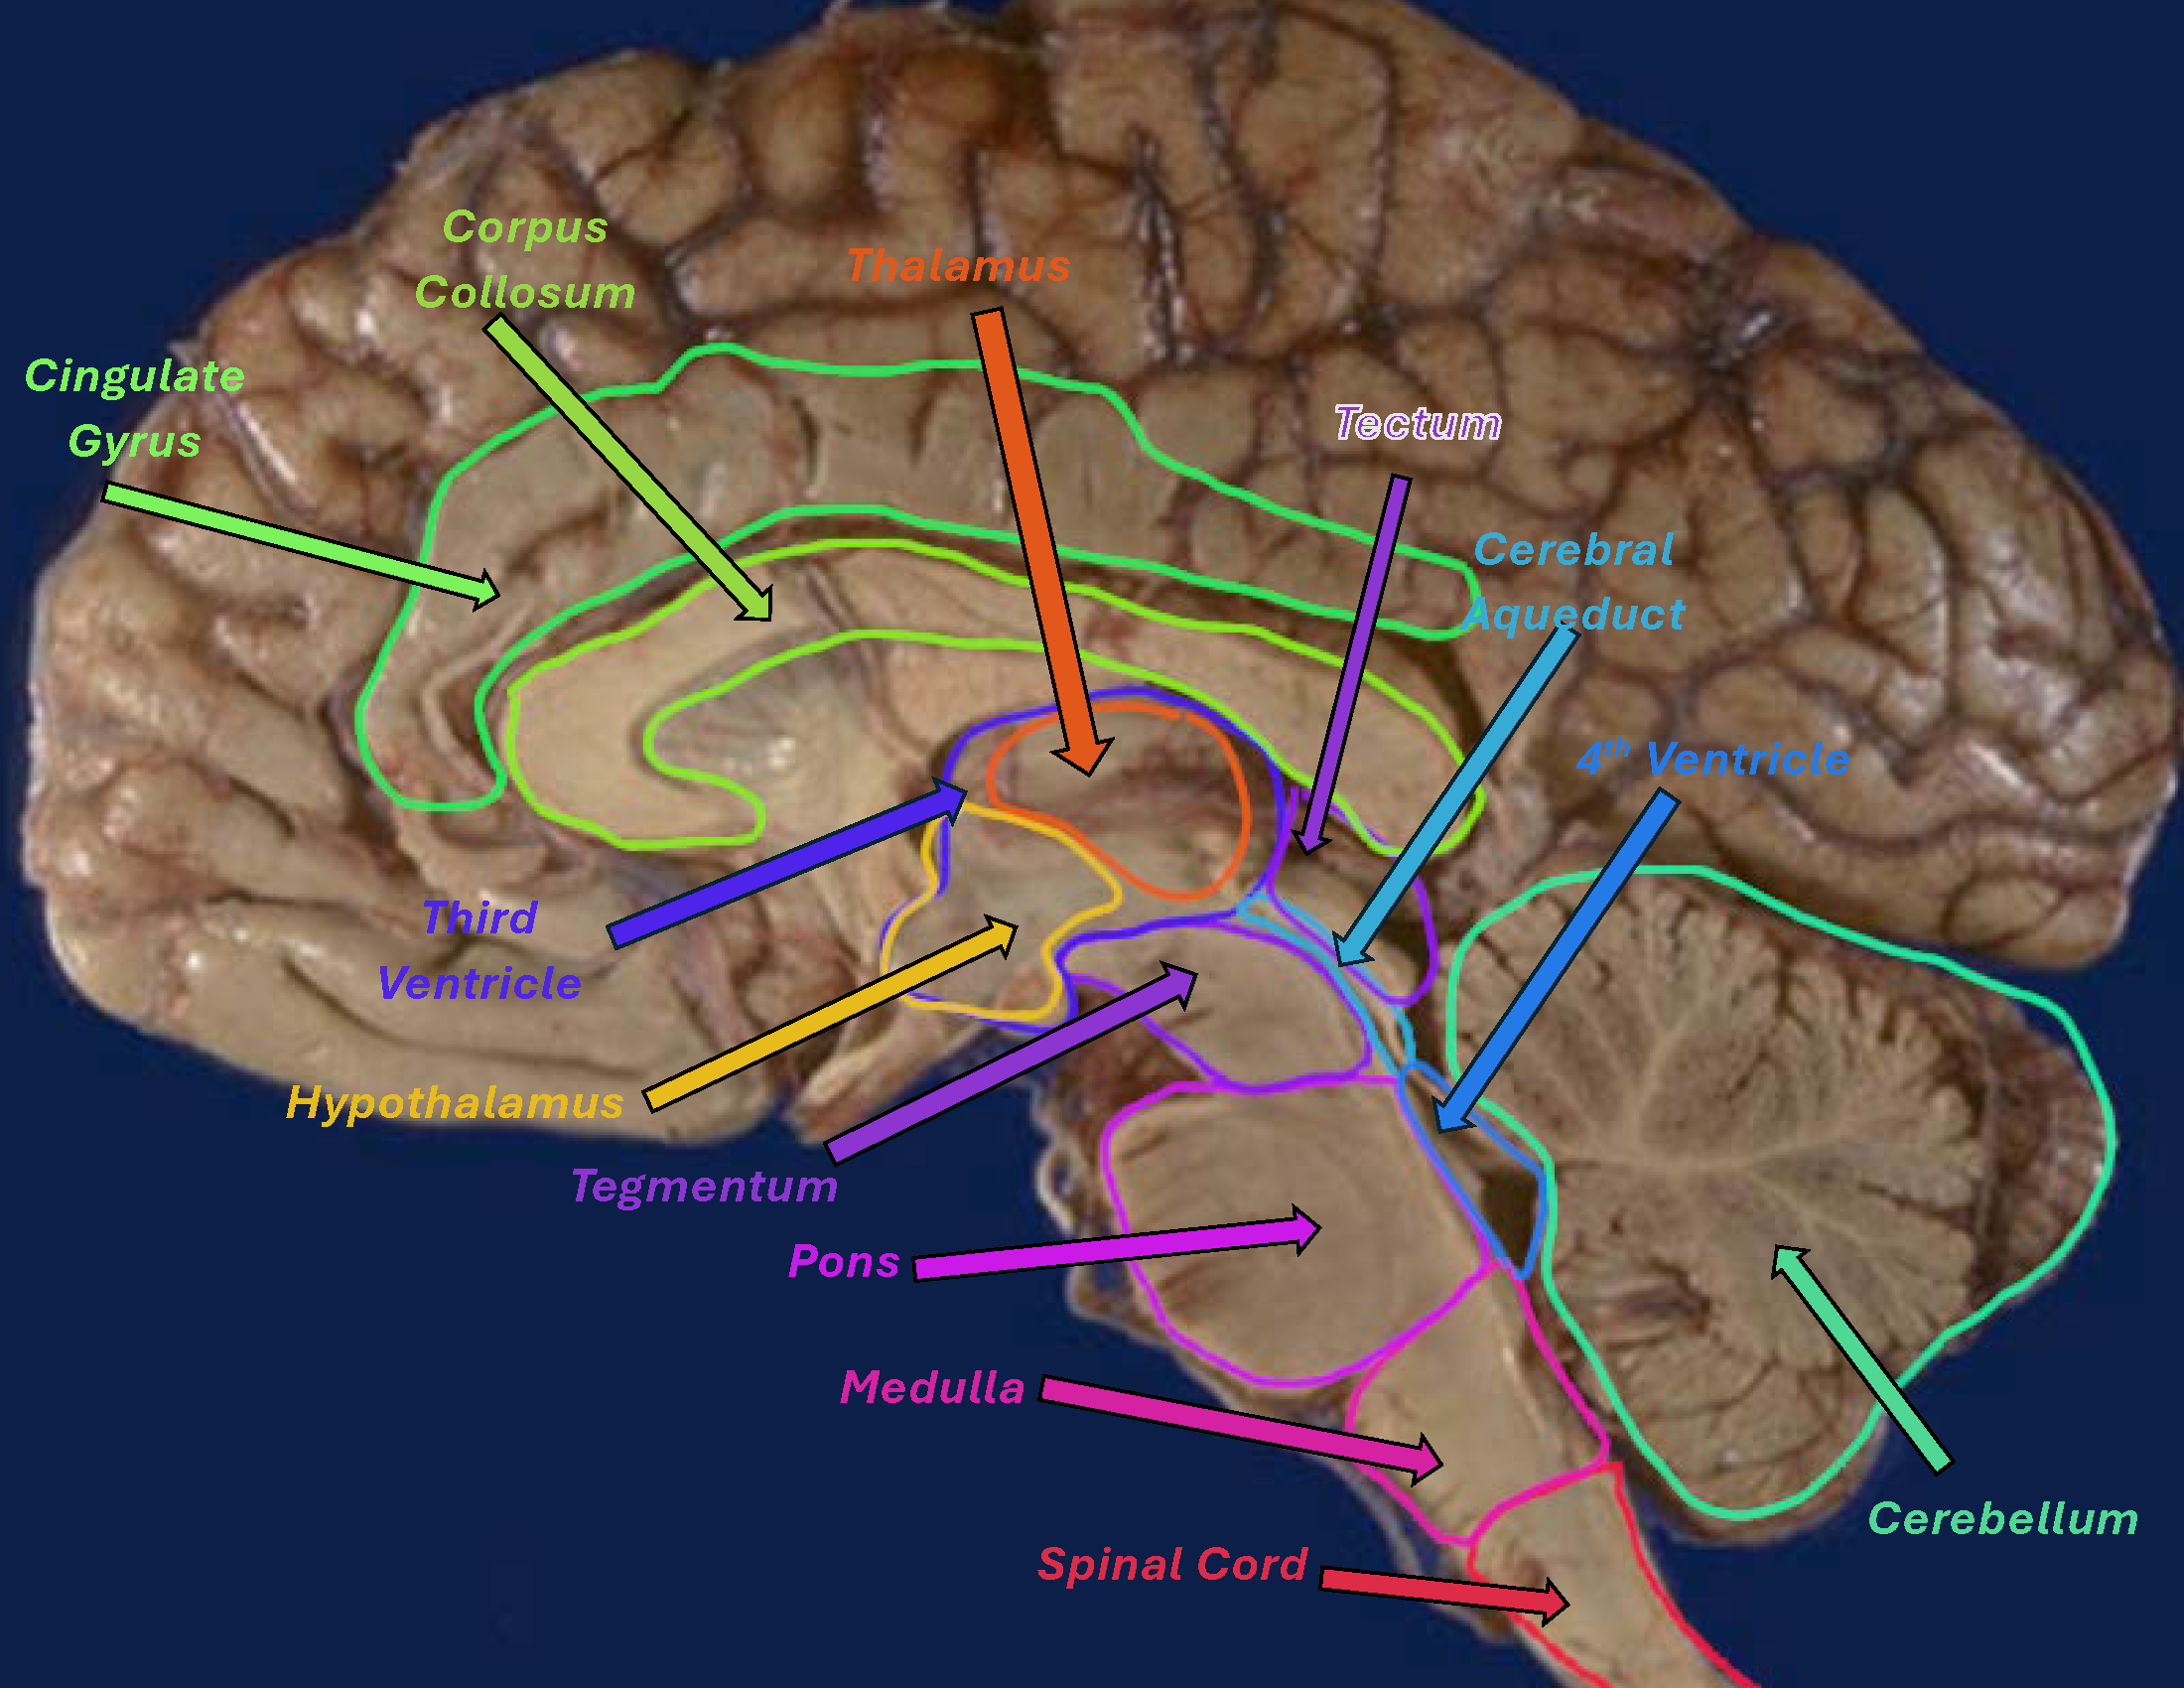
\includegraphics[width=.95\paperwidth,height=.95\paperheight,keepaspectratio]{images/midsagital_labeled.png}
%   \end{landscape}